\section{The {\em \shortname} Protocol}\label{sect:model}



%This sections describes the \shortname model as regards both the technical details and the requirements for the economic incentives.


\begin{figure}[tp]
\centering
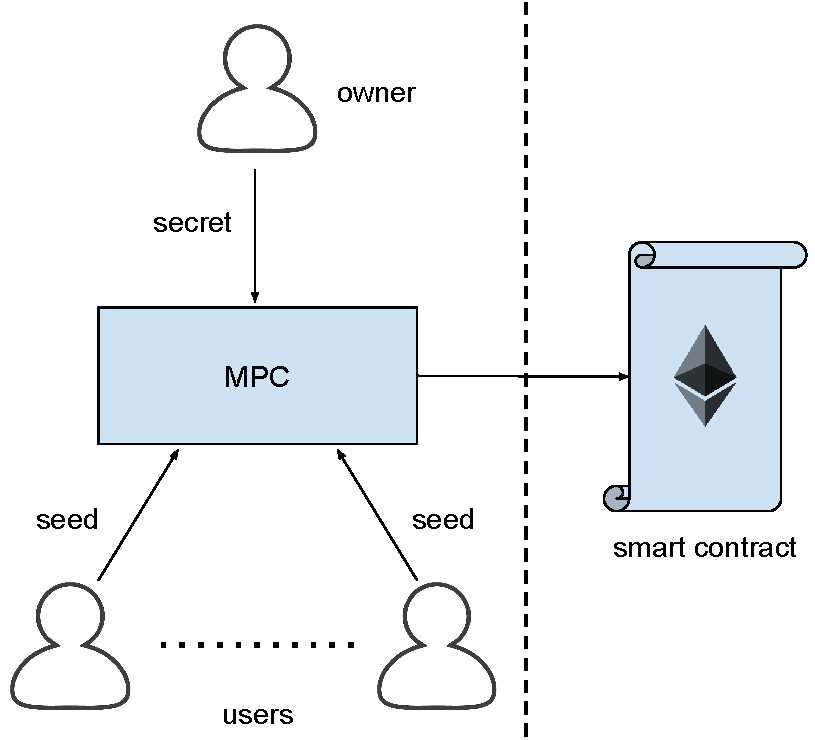
\includegraphics[width=0.6\columnwidth]{fig/proposal}
\caption{\name reference diagram}
\label{fig:model}
\end{figure}

\subsection{Terminology}

We describe \shortname{}'s  protocol using the following terminology:


\para{Secret}
A secret \secret represents the information to be protected.

\para{Time-Lock ({\em TL})}
%
A \textit{Time-Lock} is a mechanism that keeps the secret \secret private until its {\em disclosure time} \td.
%
The \textit{Time-Lock} publishes \secret{}  after \td.

\para{Owner}
An owner \owner is someone who wraps a secret \secret using a Time-Lock.
%
The owner delegates the disclosure of \secret to the Time-Lock, i.e., the owner is \textit{not} involved in the disclosure of \secret at \td.


% By creating the Time-Lock, the owner delegates the disclosure of the secret to the TL, thus effectively decoupling himself from the disclosure process (i.e., the secret will be revealed at \td without requiring the owner to play an active role in the process after the setup).

%\begin{description}
%
%	\smallskip
%    \item [Secret] --- A secret \secret represents the information to be protected.
%
%	\smallskip
%    \item [Time-Lock ({\em TL})] --- A Time-Lock is a mechanism used to keep the secret \secret private until its {\em disclosure time} \td and then publish it unconditionally.
%
%	\smallskip
%    \item [Owner] --- The owner \owner is someone who wants to wrap a secret \secret using the Time-Lock. By creating the Time-Lock, the owner delegates the disclosure of the secret to the TL, thus effectively decoupling himself from the disclosure process (i.e., the secret will be revealed at \td without requiring the owner to play an active role in the process after the setup).
%
%\end{description}
%\smallskip

\subsection{Overview}

\mg{Move this paragraph somewhere else? At this point, the reader should already have been convinced that ITYT is a meaningful approach.}
As described in Section~\ref{sect:introduction}, there are two natural implementations of a TL mechanism: the use of a trusted third-party, or the use of a Time-Lock puzzle based on the Proof-of-Work abstraction to prove the elapse of time.
%
A trusted third-party is often not acceptable, since the owner should completely entrust a single user.
On the other hand, the use of Time-Lock puzzles have been proved inadequate on different levels (e.g., assumptions on computing power in the future, waste of computing resources, incentives for the user that perform the process of decrypting the resource). \mr{tutte cose già dette}

\shortname implements a Time-Lock by distributing the secret \secret among several users so that no single user has access to \secret before the disclosure time \td.

%Concretely, the secret \secret is split into \N shares \share using Shamir's secret sharing~\cite{Shamir:1979:SS:359168.359176}.
%%
%Each share is entrusted to a \textit{shareholder} \shareholder.
%
%
%in such a way that it is possible to reconstruct \secret by combining \K different shares (i.,e., using Shamir's method~\cite{Shamir:1979:SS:359168.359176}).


\begin{description}

	\smallskip
    \item [Share] --- The secret \secret is divided into \N shares ${\share}_1,\dots,{\share}_n$ in such a way that it is possible to reconstruct \secret by combining \K different shares (i.,e., using Shamir's method~\cite{Shamir:1979:SS:359168.359176}).

	\smallskip
    \item [Shareholder] --- A shareholder \shareholder is the subject entrusted to store a share in such a way that no other party can access it before the disclosure time. After \td, the shareholders publish their shares so that anyone can reconstruct the secret \secret.

\end{description}

We propose to realize a TL mechanism by defining a protocol among the owner and the shareholders involved parties and by defining economic constraints based on the assumption that all of them will behave as rational actors.

This way, by enforcing the dynamics of the overall system, we are able to deploy an effective and practical TL mechanism.
Summarily, we propose to change the perspective from the production of a TLE scheme, \mr{non siamo mai consistenti con noi stessi nell'uso di TL e TLE} to the realization of a protocol that offer TL as the logical consequence of the protocol itself.

\mg{What is the point of the last 5 paragraphs? Presenting an overview of the protocol? Justifying our design choices?}

\mg{I guess that owner \owner and shareholders \shareholder all have keys? If yes, it's worth mentioning it somewhere.}

\subsection{Model}

\newcommand{\users}{{\ensuremath{\mathcal{U}}}\xspace}
\newcommand{\wallet}[1]{\mathit{wlt}(#1)}

\para{Time-Lock abstraction}
%
A \textit{Time-Lock} (TL) is a mechanism that keeps a secret \secret private until its {\em disclosure time} \td. \mr{Se è la prima volta che lo diciamo è troppo tardi, se lo abbiamo già detto non ripetiamolo anche qua}
%
The \textit{Time-Lock} publishes \secret{}  after \td.


\para{\shortname overview}
\shortname implements a Time-Lock by distributing the secret \secret among several users (using Shamir secret sharing~\cite{Shamir:1979:SS:359168.359176}), so that single users cannot access  \secret before the disclosure time \td.
%
\shortname introduces economic incentives and dis-incentives for the involved parties to ensure that (i) each user keeps its share secret until \td, and (ii) 
users disclose the shares and reconstruct the secret after \td.
%
As we show in Section~\ref{??}, if the users involved in \shortname's protocol behave as rational economic agents, then \shortname effectively implements the TL abstraction.
%
Rather than relying on trusted third parties~\cite{?} or Proof-of-Work~\cite{?}, \shortname implements a TL in a distributed fashion by relying on economic incentives.
\mr{quinta volta che leggo questa frase}

\mg{Can we merge the below sentence somewhere?}
%
This way, by enforcing the dynamics of the overall system, we are able to deploy an effective and practical TL mechanism.
Summarily, we propose to change the perspective from the production of a TLE scheme, to the realization of a protocol that offer TL as the logical consequence of the protocol itself.




\para{Users}
%
We denote by \users the set of users that may participate in the \shortname protocol.
%
Each user $u \in \users$ is associated with a wallet $\wallet{u}$, accessible only by $u$, that can be used to deposit or perform payments.
%
In \shortname, each user $u \in \users$ may \mg{play?}  one (or more) of the following roles:
\begin{asparaitem}
\item {\bf Owner:}	An owner \owner is someone who wraps a secret \secret using a Time-Lock.
%
The owner delegates the disclosure of \secret to the Time-Lock, i.e., the owner is \textit{not} involved in the disclosure of \secret at \td. \mr{owner already introduced in sect 3.1. We should merge them and let the owner definition appear only once}
%
In \shortname, the owner \owner sets up the TL as well as the corresponding parameters.
%
In particular, \owner sets (i) \N, i.e., the total number of shares $h_i$ of \secret, (ii) $k$, i.e., the number of shares needed to recover \secret, and (iii) the rewards that must be paid to the shareholders \shareholder and to the whistleblower \whistleblower.
%
Next, \owner splits the secret  \secret  into \N shares $\share_1,\dots,\share_n$ using Shamir $k$-out-of-\N secret sharing~\cite{Shamir:1979:SS:359168.359176}.

\item {\bf Shareholder:}
%
A shareholder \shareholder is entrusted by the owner \owner to store a share \share of the secret \secret. 
%
The shareholder should keep the share \share secret until \td, and disclose \share after \td.
%
Whenever the protocol is correctly executed, i.e., the secret \secret is disclosed only after \td, the shareholder receives a remuneration.

\item {\bf Whistleblower:}
%
A whistleblower \whistleblower reports misbehaviors in the execution of the protocol in exchange for an economic incentive.
%
Whenever \whistleblower possesses \secret before \td, \whistleblower can report this and receive a compensation.
%
Observe that only if a coalition of $k$ (malicious?) shareholders collude to reconstruct \secret before \td. \mr{l'ultima frase non l'ho capita}
\end{asparaitem}


\para{\shortname Protocol}
%
\shortname consists of three sub-protocols: the {\em setup},  {\em disclosure} and  {\em whistleblowing} protocols.
%
Next, we describe each of these subprotocols.






\subsection{Protocol description}

\shortname consists of the {\em setup},  {\em disclosure} and  {\em whistleblowing} protocols.

\paragraph{The setup protocol}

\begin{figure}[t]
\centering
\protocol{Setup Protocol}{
\begin{enumerate}
	\item The owner defines all the parameters for the time-lock (i.e., the disclosure time \td, and the economic incentives)
	\item The owner deposits her payment \PO, along with \N shares \share (one for each shareholder \shareholder) of the secret \secret.
	\item The owner publish a commitment of the secret \Csecret and a commitment for each share \Cshare{i}.
	\item Each shareholder $\shareholder_{i}$, deposits a bid \BH and receives the share $\share_{i}$ of the secret \secret that she has to protect.
	\item When all the shareholders have claimed their shares, the setup is completed and the time-lock is enforced. If something goes wrong during the setup, the owner's payment and the already paid shareholder bids are released to their respective owners.
\end{enumerate}
}
\caption{\shortname setup protocol}
\label{protocol:setup}
\end{figure}

\shortname is implemented by modeling the interaction of a secret owner \owner, and by \N shareholders \shareholder. \owner aims at securely storing the secret \secret, whose value is estimated to be \V, and at disclosing it at \td.
%
By splitting the secret \secret in \N shares $\share_{1},\ \ldots,\ \share_{\N}$, the owner does not have to entrust a single third-party that would be able to know \secret before \td. By leveraging threshold cryptography, the owner enforces that \K-of-\N shareholders are required to cooperate to disclose the secret.

To be able to use the TL service, the owner is willing to pay an amount \PO. A shareholder \shareholder is instead incentivized to take part to a TL protocol by the possibility of earning a reward \RH. However, to demonstrate his goodwill, each shareholder is asked to deposit a bid \BH in order to retrieve his share.
%
The phases of the setup protocol are illustrated in Figure~\ref{protocol:setup}.

\paragraph{The disclosure protocol}

In case of correct execution of the protocol (the secret does not leak before \td),  \owner is able to fulfill his promise to all the shareholders by distributing \PO such that a reward \RH is paid to each shareholder that publishes her share, thus each of them obtains a profit $\profit = \RH - \BH > 0$.

We can define the owner's payment to be:

\begin{equation}\label{eqbalance}
\PO = \N \cdot \profit
\end{equation}

When \K shares have been published, anyone is able to retrieve the original secret, thus effectively unlocking the TL.

The phases of the disclosure protocol are illustrated in Figure~\ref{protocol:disclosure}.

\begin{figure}[t]
	\centering
	\protocol{Disclosure Protocol (after \td, executed once per share $\share_{i}$)}{
		\begin{enumerate}
			\item A user $\mathcal{U}$ (usually the shareholder $\shareholder_{i}$) publishes the share $\share_{i}$.
			\item If $\share_{i}$ has already been published or does not match the commitment \Cshare{i}, the disclosure protocol fails and terminates. \mrosa{e se uno sbaglia, termina subito tutto?}
			\item The submitted share is marked as published, and the shareholder reward is transferred to the submitting user $\mathcal{U}$.
			\item If this is the first submitted share for the \shortname protocol, the owner reward \RO is transferred to the owner \owner. \mrosa{bisogna spiegare nel testo perche' anche l'owner riceve qualcosa indietro}
		\end{enumerate}
	}
	\caption{\shortname disclosure protocol}
	\label{protocol:disclosure}
\end{figure}

\paragraph{The whistleblowing protocol}

To disincentivize misbehavior, in the event that the secret is reconstructed before \td from a malicious coalition composed by at least \K shareholders, we introduce an economic penalization. In particular, each shareholder participating in the protocol is subjected to an economic penalty that results in the loss of the payment/bid already paid.

However, if all the subjects involved in the TL protocol were punished, then nobody would have an incentive to unveil an attack.
% Another problem is that a mechanism like the one presented has nor control nor enforcement over the state of execution, because \secret could be valuable for someone that does not require the secret to be disclosed to the public; thus the secret might be used outside the circuit and the revenue could still be gathered.
%qua ci vorrebbe una citazione famosa a caso a proposito delle spie o dei traditori per spezzare il discorso, bisogna introdurre il ruolo del whistleblower che é necessario come contrappeso
In order to make the mechanism work, it is then required to introduce a proper countermeasure, in particular a new role can be introduced in our model: the {\em whistleblower} \whistleblower, i.e., someone interested in proving the possession of \secret before the disclosure time.

%It is also required for the participants to compete for the whistleblower role, so that 
The first party able to prove the attack is rewarded with the whistleblower bonus \Wbonus. If the whistleblowing protocol succeeds, the \shortname protocol is considered failed, and no more actions are allowed.
%
The whistleblowing protocol is detailed in Figure~\ref{protocol:whistleblowing}.

\begin{figure}[t]
	\centering
	\protocol{Whistleblowing Protocol (before \td)}{
		\begin{enumerate}
			\item A user \whistleblower publishes a secret $\secret'$ after the time-lock entered the enforced state but before \td has passed.
			\item If the published secret $\secret'$ does not match the commitment \Csecret, the whistleblower protocol fails and terminates.
			\item Else, the whistleblower bonus \Wbonus is transferred to the whistleblower \whistleblower; the \shortname protocol is marked as failed and no further actions are processed (the remaining funds are lost).
		\end{enumerate}
	}
	\caption{\shortname whistleblowing protocol}
	\label{protocol:whistleblowing}
\end{figure}
